\chaptertitlepage{Results and Discussion}

This chapter reports how the four-class system performed on the held-out test split of \path{training/manifest.csv}. Every accuracy, precision, recall, F1, confusion-matrix, and leakage-probe figure comes from the evaluation exports (\path{training/results/comparison.md}, \path{results.json}, \path{ensemble.json}, \path{leakage_probe.json}) and the run logs. Scores from the earlier single-disease models appear only in their own section, labelled as prior work, and never in the four-class tables.

\section{Experimental Setup}

We used seed 1337, patient-grouped splits, and the class order Normal, Tuberculosis, COVID-19, Pneumonia. The splits came out at 2{,}260 training, 485 validation, and 482 test images (70.0\%, 15.0\%, and 14.9\%). All models were trained with a batch size of 32 and inverse-frequency class weights (COVID-19 weight $\approx$ 2.851), and each class was capped at 1{,}200 images for this run (\texttt{--cap 1200}).

\begin{table}[H]
\centering
\caption{Training environment (machine that produced the four-class weights)}
\label{tab:env-train}
\small
\begin{tabular}{@{}P{4.0cm}P{8.2cm}@{}}
\toprule
\HeaderRow \Head{Item} & \Head{Value} \\
\midrule
OS & macOS 15.7.9 (x86\_64) \\
\ZebraRow CPU & Intel Core i9-9980HK @ 2.40\,GHz (16 logical cores) \\
Memory & 32\,GB \\
\ZebraRow GPU & None (CPU-only TensorFlow) \\
Python / TensorFlow / Keras & 3.11.15 / 2.16.2 / 3.15.0 \\
\ZebraRow Training dates & DenseNet121: 4 Aug 2026; EfficientNetB3: 5 Aug 2026; CNN: 9 Aug 2026 \\
Evaluation & Per-model comparison: 9 Aug 2026; ensemble + leakage: 13 Sep 2026 \\
\bottomrule
\end{tabular}
\end{table}

\section{Unified Manifest Summary}

Removing duplicates by MD5 content hash took out 45 images and left a pool of 10{,}328. COVID-19 dropped from 137 to 130 images. The manifest selected from this pool has 3{,}227 images. The COVID source's Viral Pneumonia images are counted as Pneumonia, which is where the 89 \texttt{covid\_db} images in that class come from.

\begin{table}[H]
\centering
\caption{Selected unified manifest counts by class and split}
\label{tab:manifest-splits}
\small
\begin{tabular}{@{}lrrrr@{}}
\toprule
\HeaderRow \Head{Class} & \Head{Train} & \Head{Val} & \Head{Test} & \Head{Total} \\
\midrule
Normal & 840 & 180 & 180 & 1{,}200 \\
\ZebraRow Tuberculosis & 488 & 105 & 104 & 697 \\
COVID-19 & 91 & 20 & 19 & 130 \\
\ZebraRow Pneumonia & 841 & 180 & 179 & 1{,}200 \\
\AccentRow \textbf{Total} & \textbf{2{,}260} & \textbf{485} & \textbf{482} & \textbf{3{,}227} \\
\bottomrule
\end{tabular}
\end{table}

\begin{table}[H]
\centering
\caption{Class $\times$ source contingency (selected manifest)}
\label{tab:class-source}
\small
\begin{tabular}{@{}lrrrr@{}}
\toprule
\HeaderRow \Head{Class} & \Head{covid\_db} & \Head{pneumonia\_db} & \Head{tb\_db} & \Head{Total} \\
\midrule
Normal & 88 & 556 & 556 & 1{,}200 \\
\ZebraRow Tuberculosis & 0 & 0 & 697 & 697 \\
COVID-19 & 130 & 0 & 0 & 130 \\
\ZebraRow Pneumonia & 89 & 1{,}111 & 0 & 1{,}200 \\
\AccentRow \textbf{Total} & \textbf{307} & \textbf{1{,}667} & \textbf{1{,}253} & \textbf{3{,}227} \\
\bottomrule
\end{tabular}
\end{table}

Normal and Pneumonia draw on several datasets by design. Tuberculosis and COVID-19 each come from a single dataset, so a model could more easily learn to recognise them by their source (Section~\ref{sec:leakage}).

\section{Four-Class Comparative Results}

All models were scored on the same test split ($n=482$). The ensemble figures come from the offline \texttt{ensemble.json}, which averages the three models' class probabilities.

\begin{table}[H]
\centering
\caption{Overall four-class test metrics ($n=482$)}
\label{tab:comparative}
\small
\begin{adjustbox}{max width=\textwidth}
\begin{tabular}{@{}lccccc@{}}
\toprule
\HeaderRow \Head{Model} & \Head{Accuracy} & \Head{Bal.\ Acc.} & \Head{Macro P} & \Head{Macro R} & \Head{Macro F1} \\
\midrule
EfficientNetB3 & 82.99\% & 83.00\% & 0.767 & 0.830 & 0.745 \\
\ZebraRow DenseNet121 & 90.87\% & 89.14\% & 0.850 & 0.891 & 0.864 \\
Custom CNN & 90.25\% & 88.36\% & 0.813 & 0.884 & 0.835 \\
\AccentRow Ensemble (soft vote) & \textbf{92.32\%} & \textbf{93.07\%} & 0.842 & \textbf{0.931} & \textbf{0.867} \\
\bottomrule
\end{tabular}
\end{adjustbox}
\end{table}

DenseNet121 is the best single model on accuracy (90.87\%), balanced accuracy (89.14\%), and macro F1 (0.864). EfficientNetB3 has the highest COVID-19 recall of the three (89.47\%), but its COVID-19 precision is much lower. Combining the models lifts accuracy to 92.32\% and balanced accuracy to 93.07\%.

We treat balanced accuracy as the main metric. COVID-19 has only 19 test images, so plain accuracy would barely register how well the models handle it.

\section{Per-Class Precision, Recall, and F1}

\subsection{Recall summary}

\begin{table}[H]
\centering
\caption{Per-class recall on the test set}
\label{tab:recall}
\small
\begin{tabular}{@{}lcccc@{}}
\toprule
\HeaderRow \Head{Model} & \Head{Normal} & \Head{TB} & \Head{COVID-19} & \Head{Pneumonia} \\
\midrule
EfficientNetB3 & 78.3\% & 69.2\% & 89.5\% & 95.0\% \\
\ZebraRow DenseNet121 & 86.1\% & 88.5\% & 84.2\% & 97.8\% \\
Custom CNN & 80.6\% & 96.2\% & 78.9\% & 97.8\% \\
\AccentRow Ensemble & 85.6\% & 94.2\% & 94.7\% & 97.8\% \\
\bottomrule
\end{tabular}
\end{table}

\subsection{DenseNet121 (best single-model macro F1)}

\begin{table}[H]
\centering
\caption{DenseNet121 per-class metrics}
\label{tab:densenet-pc}
\small
\begin{tabular}{@{}lcccc@{}}
\toprule
\HeaderRow \Head{Class} & \Head{Precision} & \Head{Recall} & \Head{F1} & \Head{Support} \\
\midrule
Normal & 92.3\% & 86.1\% & 0.891 & 180 \\
\ZebraRow Tuberculosis & 97.9\% & 88.5\% & 0.929 & 104 \\
COVID-19 & 59.3\% & 84.2\% & 0.696 & 19 \\
\ZebraRow Pneumonia & 90.7\% & 97.8\% & 0.941 & 179 \\
\bottomrule
\end{tabular}
\end{table}

\subsection{Ensemble (soft voting)}

\begin{table}[H]
\centering
\caption{Ensemble per-class metrics}
\label{tab:ensemble-pc}
\small
\begin{tabular}{@{}lcccc@{}}
\toprule
\HeaderRow \Head{Class} & \Head{Precision} & \Head{Recall} & \Head{F1} & \Head{Support} \\
\midrule
Normal & 95.7\% & 85.6\% & 0.903 & 180 \\
\ZebraRow Tuberculosis & 97.0\% & 94.2\% & 0.956 & 104 \\
COVID-19 & 48.7\% & 94.7\% & 0.643 & 19 \\
\ZebraRow Pneumonia & 95.6\% & 97.8\% & 0.967 & 179 \\
\bottomrule
\end{tabular}
\end{table}

COVID-19 precision is low for every model, and no single model gets above about 60\%. The ensemble's COVID-19 recall of 94.7\% looks strong, but it rests on only 19 test cases ($n=19$) and could shift noticeably on a different sample, so it should always be quoted with that caveat.

\section{Confusion Matrices}

In each matrix the rows are the true classes and the columns the predicted classes, both in the order Normal, Tuberculosis, COVID-19, Pneumonia.

\begin{figure}[H]
\centering
\begin{minipage}{0.48\textwidth}
\centering
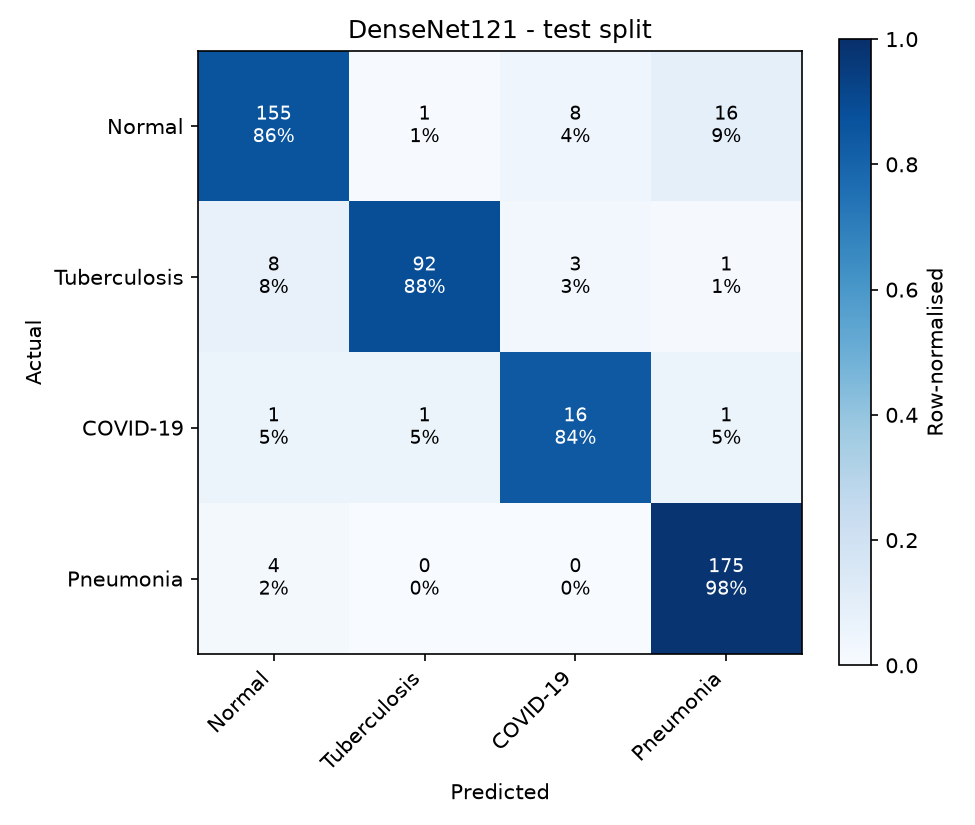
\includegraphics[width=\linewidth]{images/results/confusion_densenet.png}
\caption{DenseNet121 confusion matrix}
\label{fig:cm-densenet}
\end{minipage}\hfill
\begin{minipage}{0.48\textwidth}
\centering
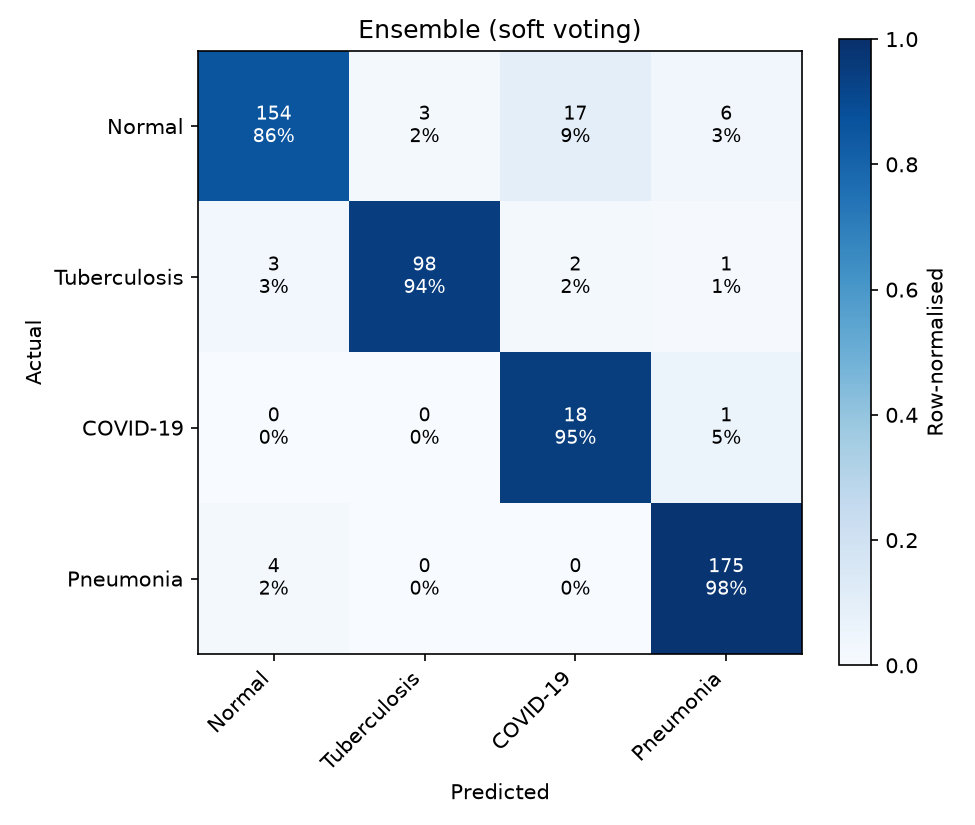
\includegraphics[width=\linewidth]{images/results/confusion_ensemble.png}
\caption{Ensemble confusion matrix}
\label{fig:cm-ensemble}
\end{minipage}
\end{figure}

\begin{figure}[H]
\centering
\begin{minipage}{0.48\textwidth}
\centering
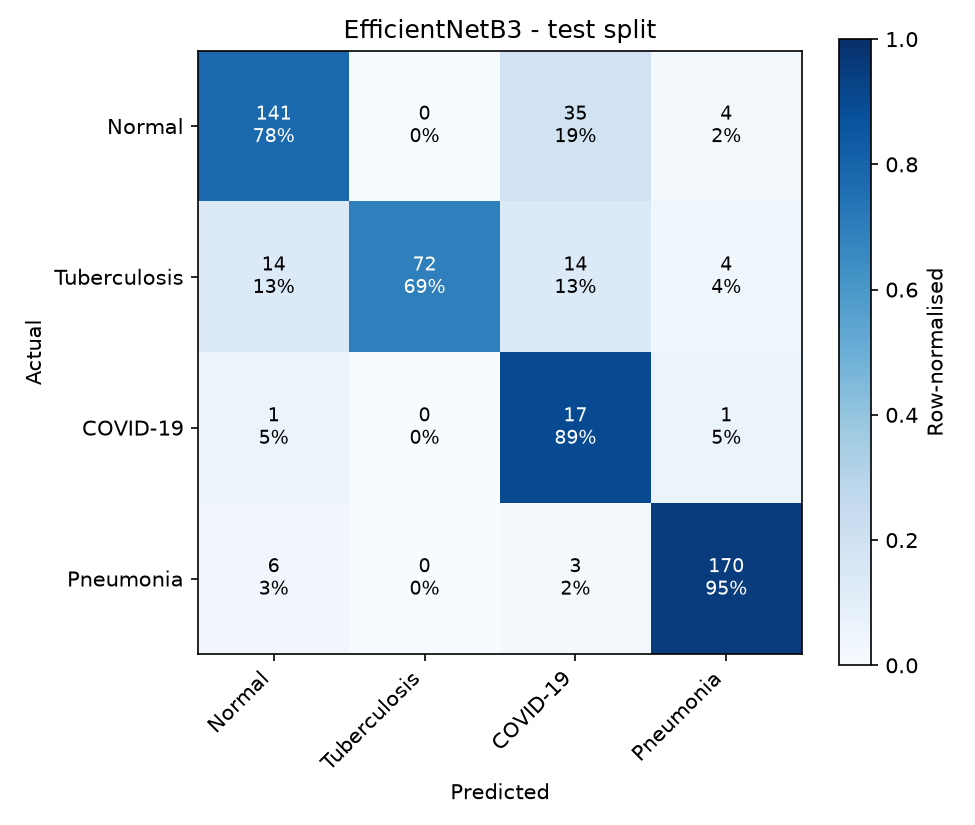
\includegraphics[width=\linewidth]{images/results/confusion_efficientnet.png}
\caption{EfficientNetB3 confusion matrix}
\label{fig:cm-efficientnet}
\end{minipage}\hfill
\begin{minipage}{0.48\textwidth}
\centering
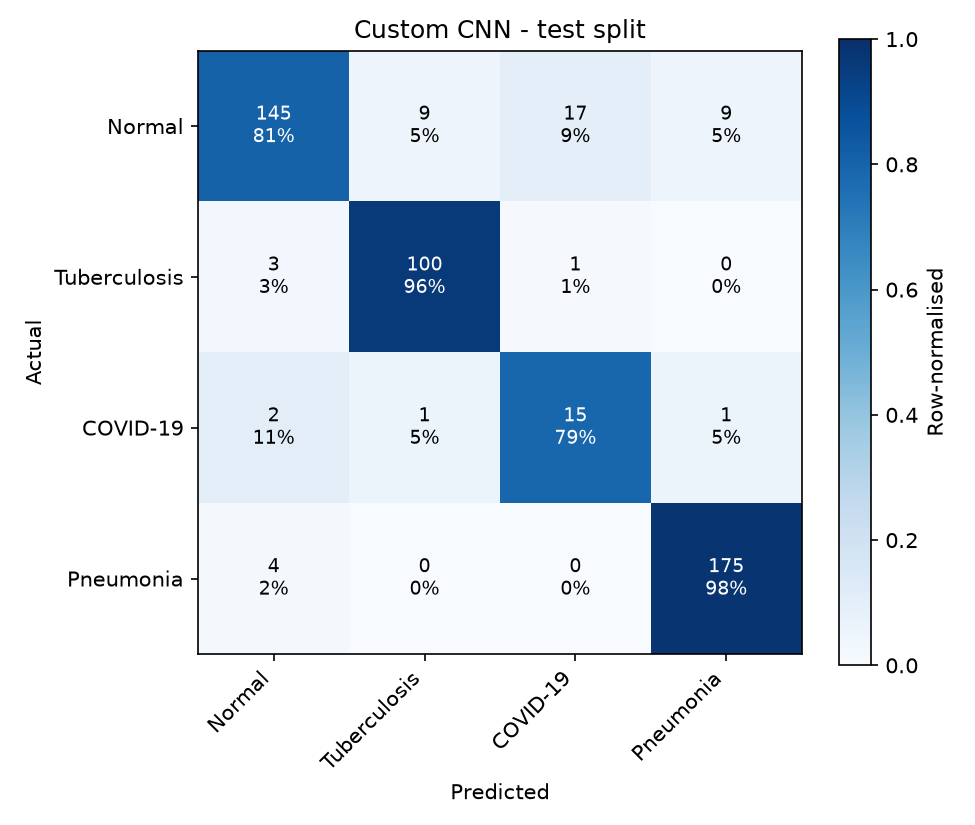
\includegraphics[width=\linewidth]{images/results/confusion_cnn.png}
\caption{Custom CNN confusion matrix}
\label{fig:cm-cnn}
\end{minipage}
\end{figure}

\section{Leakage Probe}
\label{sec:leakage}

The probe is a custom CNN at $150\times150$, trained for 8 epochs to predict which dataset each image came from. It named the source correctly 88.17\% of the time, against a majority-class baseline of 49.79\%, a gap of 38.4 percentage points. We rate this as a moderate source signal: the datasets can partly be told apart by source, though far from perfectly. Because Tuberculosis and COVID-19 each come from a single dataset, part of their recall may rest on scanner or processing cues. Normal and Pneumonia come from several datasets and are less exposed to that shortcut. The disease results earlier in this chapter should be read with this caveat in mind.

\section{Training Run Summary}

\begin{table}[H]
\centering
\caption{Saved validation metrics and training cost}
\label{tab:runs}
\small
\begin{adjustbox}{max width=\textwidth}
\begin{tabular}{@{}lcccc@{}}
\toprule
\HeaderRow \Head{Model} & \Head{Val Acc.} & \Head{Val Loss} & \Head{Epochs} & \Head{Train time} \\
\midrule
EfficientNetB3 & 80.00\% & 0.492 & 20 & $\sim$35.7\,h (CPU) \\
\ZebraRow DenseNet121 & 89.90\% & 0.299 & 20 & 310.6\,min \\
Custom CNN & 88.87\% & 0.354 & 20 & 36.8\,min \\
\bottomrule
\end{tabular}
\end{adjustbox}
\end{table}

The models have roughly 11.2\,M (EfficientNetB3), 7.3\,M (DenseNet121), and 1.25\,M (custom CNN) parameters. EfficientNetB3 took so long to train because the Mac we used had no GPU, so it trained on the CPU alone.

\section{Deployed Interface Demonstrations}

Figures~\ref{fig:tb-prediction} to~\ref{fig:pneumonia-prediction} show the Flask interface returning soft-voting verdicts on which all three models agree, with each model's probability bars. The application combines the models with the same soft-voting rule used in the offline evaluation above.

\begin{figure}[H]
\centering
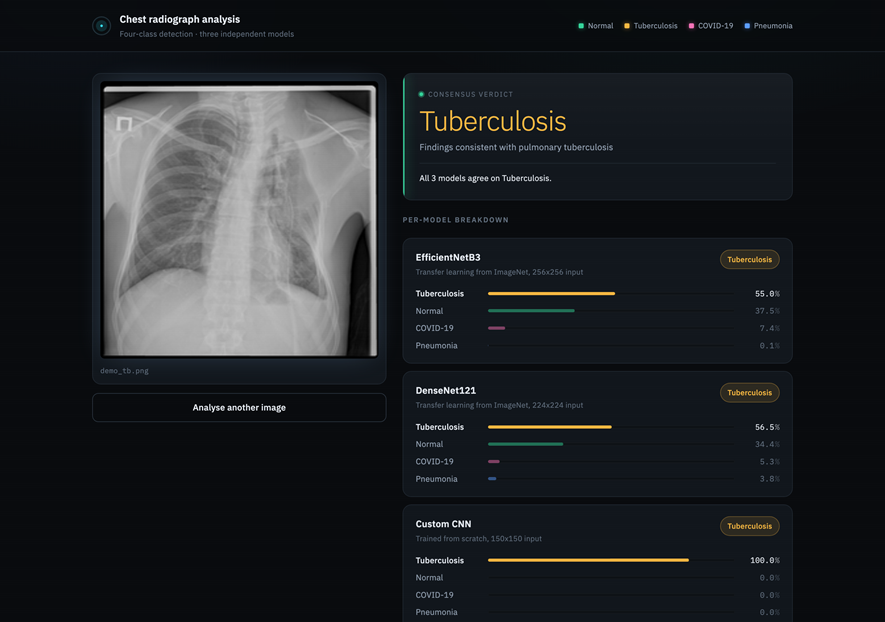
\includegraphics[width=0.92\textwidth]{images/ui_tb_result.png}
\caption{Consensus Tuberculosis verdict with per-model 4-class probability bars}
\label{fig:tb-prediction}
\end{figure}

\begin{figure}[H]
\centering
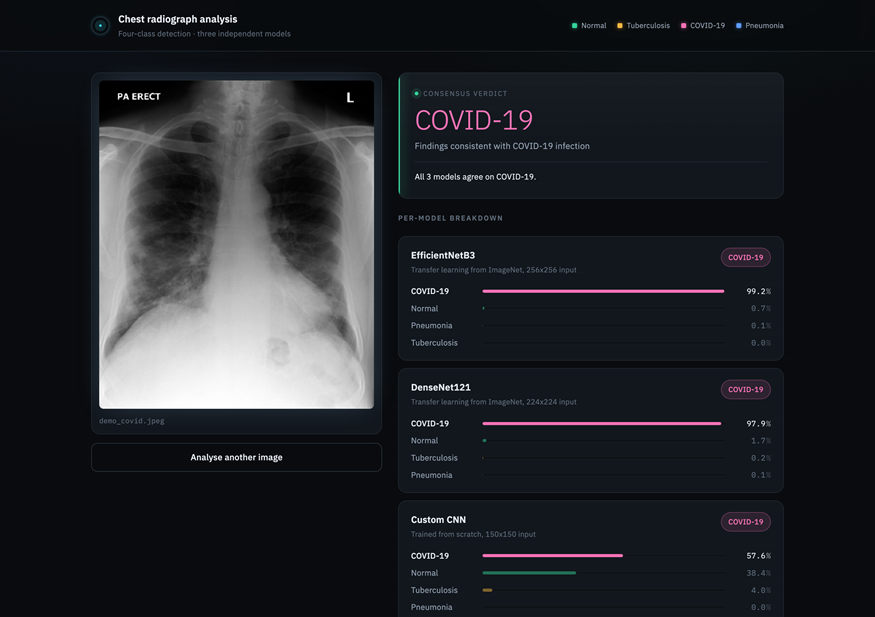
\includegraphics[width=0.92\textwidth]{images/ui_covid_result.png}
\caption{Consensus COVID-19 verdict with per-model 4-class probability bars}
\label{fig:covid-prediction}
\end{figure}

\begin{figure}[H]
\centering
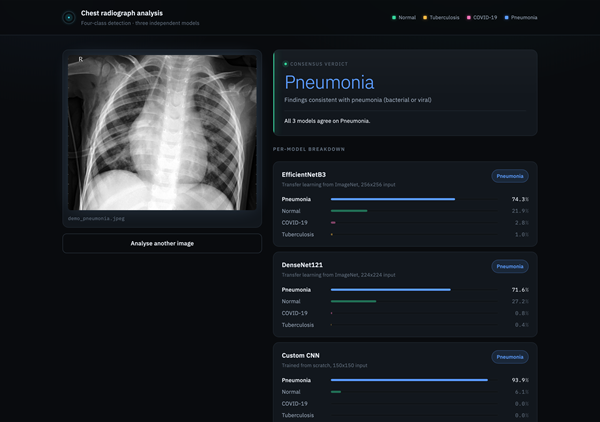
\includegraphics[width=0.92\textwidth]{images/ui_pneumonia_result.png}
\caption{Consensus Pneumonia verdict with per-model 4-class probability bars}
\label{fig:pneumonia-prediction}
\end{figure}

\section{Challenges Faced and Solutions Applied}

\begin{table}[H]
\centering
\caption{Challenges and solutions during the 4-class conversion}
\label{tab:challenges}
\footnotesize
\begin{adjustbox}{max width=\textwidth}
\begin{tabular}{@{}cP{3.8cm}P{4.8cm}@{}}
\toprule
\HeaderRow \Head{\#} & \Head{Challenge} & \Head{Solution} \\
\midrule
1 & Incomparable old models & Unified 4-class manifest \\
\ZebraRow 2 & Patient/filename leakage & Grouped IDs + hash dedupe \\
3 & Sigmoid + categorical bug & Softmax heads for all models \\
\ZebraRow 4 & Unfair fine-tune by layer index & Match $\sim$43\% unfreeze fraction \\
5 & Non-X-ray uploads & Rebuilt 3-stage gate (21\%$\rightarrow$77\% reject) \\
\ZebraRow 6 & Train/serve resize skew & Align bilinear decode \\
7 & Missing P/R/F1 historically & \texttt{evaluate.py} suite \\
\ZebraRow 8 & Small COVID set ($n{=}130$) & Class weights + honest recall/precision reporting \\
\bottomrule
\end{tabular}
\end{adjustbox}
\end{table}

\section{Historical Single-Disease Work}

Our earlier binary models scored 95.63\% test accuracy for TB (EfficientNetB3) and 92\% for pneumonia (custom CNN, on 624 test images). The old COVID-19 model overfitted so badly that its validation accuracy was near 0\%. These figures are \textbf{not comparable} with the four-class results in this chapter, and we include them only as background on how the project developed.

\section{Implementation Status}

\begin{table}[H]
\centering
\caption{Implementation status after evaluation export}
\label{tab:status}
\small
\begin{tabular}{@{}P{5.2cm}P{6.5cm}@{}}
\toprule
\HeaderRow \Head{Component} & \Head{State} \\
\midrule
Unified manifest & Complete (3{,}227 images; Table~\ref{tab:manifest-splits}) \\
\ZebraRow Four-class weights & Present \\
Held-out evaluation & Complete (Tables~\ref{tab:comparative}--\ref{tab:ensemble-pc}) \\
\ZebraRow Leakage probe & Complete (88.17\% vs 49.79\% baseline) \\
Frontend ensemble UI + gate & Complete \\
\bottomrule
\end{tabular}
\end{table}

\section{Summary of Findings}

On the four-class test set ($n=482$), DenseNet121 is the strongest single backbone (90.87\% accuracy, 89.14\% balanced accuracy, macro F1 0.864), and the soft-voting ensemble does better still, with 92.32\% accuracy and 93.07\% balanced accuracy. Every model recognises pneumonia well, with recall of at least 95\%. COVID-19 is the hard class. Its recall can be high (94.7\% for the ensemble) while precision stays low, and with only 19 COVID-19 test images neither figure is stable. The leakage probe found a moderate source signal (88.17\% against a 49.79\% baseline), so the TB and COVID-19 results, which each come from one dataset, need cautious reading. The redesign met its goal: the three architectures were compared fairly on shared data, and the per-class metrics show how the minority class performs, which overall accuracy would have hidden.
